% -*- coding: utf-8; -*-

\chapter{Geração Baseada em Derivadas Médias}
\label{ch:my}
	Este capítulo descreve o método proposto nessa dissertação para gerar funções de transferência automáticas, baseado no trabalho de \textit{Kindlmann e Durkin}~\cite{gordon}, explicado no capítulo anterior.

\section{Detecção de Fronteiras}
\label{sec:my.deriv}
	Para eliminar o problema de deslocamento em $ h(v) $ é preciso repensar o modelo de \textit{Kindlmann e Durkin}~\cite{gordon} a fim de identificar a fronteira pela segunda derivada que não seja através de $ f''(x) = 0 $. Uma opção é utilizar o ponto de inflexão que ocorre quando $ f''(x) = 0 $. No entanto, como são encontrados três pontos de inflexão ao longo de $ f''(x) $, é preciso identificar aquele que ocorre quando $ f'(x) $ é máximo.
	
	Para encontrar o ponto de inflexão de uma função, deve-se avaliar sua primeira e segunda derivadas. Na verdade, um ponto de inflexão é encontrado da mesma forma que a fronteira é identificada: um extremo local na primeira derivada e segunda derivada igual a zero. O que faz sentido, uma vez que segundo o modelo estipulado, o centro de uma fronteira é exatamente um ponto de inflexão. A Figura~\ref{fig:m_inflection} mostra $ f''(x) $ como $ D(x) $ e suas respectivas derivadas $ D'(x) $ e $ D''(x) $, onde os pontos de inflexão são indicados pelas retas tracejadas.
	
\begin{figure}[h]
	\centering
	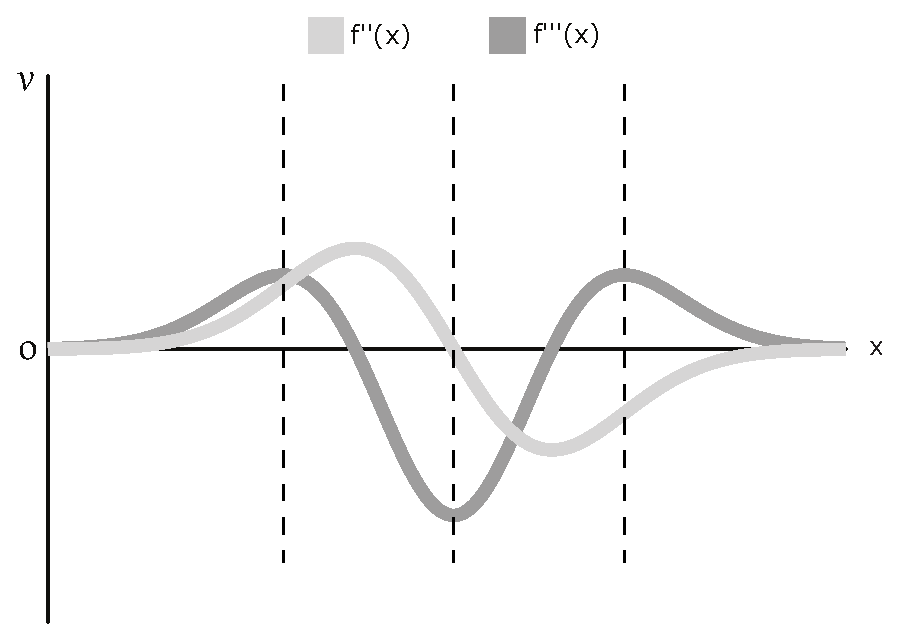
\includegraphics[width=0.7\textwidth]{images/m_inflection}
	\label{fig:m_inflection}
	%TODO
	\caption{Lalala...}
\end{figure}

	Vê-se que apenas um extremo de $ D'(x) $ é negativo. Essa informação é indiferente para encontrar os pontos de inflexão, mas é muito útil na detecção da fronteira, pois a posição do extremo negativo é justamente $ D(x) = 0 $, onde se encontra o centro da fronteira. Lembrando que $ D'(x) = f'''(x), $ percebe-se que $ f'''(x) $ pode ser utilizada no lugar de $ f''(x) $ para identificar uma fronteira, como mostra a Figura~\ref{fig:m_functions}.
	
\begin{figure}[h]
	\centering
	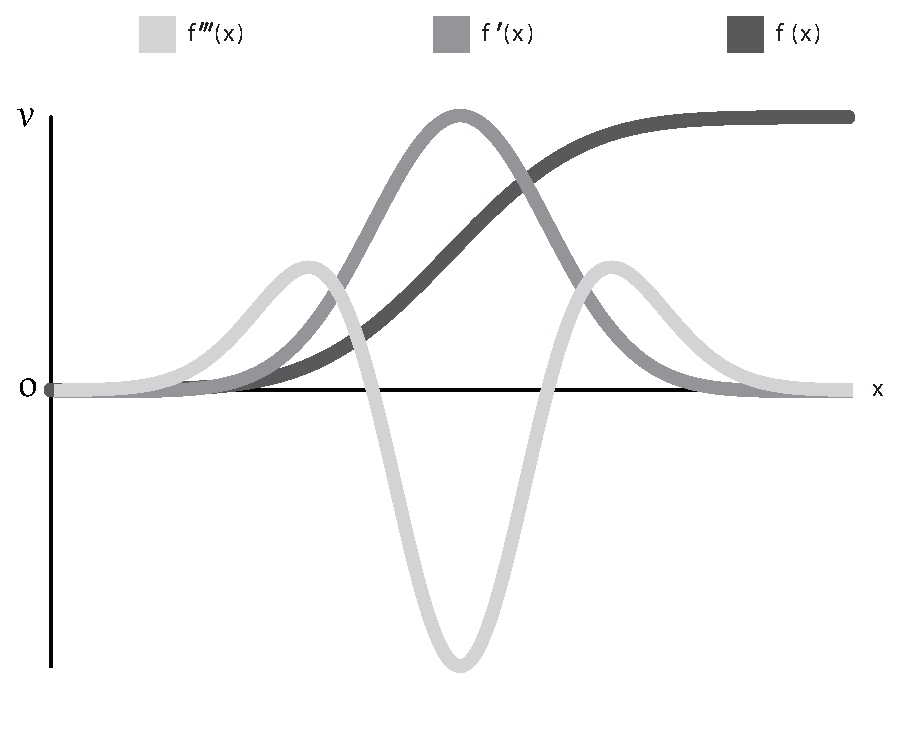
\includegraphics[width=0.7\textwidth]{images/m_functions}
	\label{fig:m_functions}
	%TODO
	\caption{Lalala...}
\end{figure}

	É preciso obter uma nova relação para extrair $ \sigma $ e $ x $, mas agora utilizando $ f'(x) $ e $ f'''(x) $. Para facilitar a leitura, $ f'(x) $ é repetida na equação~\eqref{eq:first2}, enquanto a função $ f'''(x) $ é definida na equação~\eqref{eq:third}. Devido ao fato de $ f'(x) $ ter um grande termo em comum com $ f'''(x) $, a simples divisão entre essas funções revela uma relação envolvendo $ \sigma $ e $ x $, como mostra a equação~\eqref{eq:sigmax}. Com $ x = 0 $ percebe-se que, mais uma vez, o valor de $ \sigma $ pode ser recuperado através dos valores extremos das derivadas, indicado na equação~\eqref{eq:sigma3}. Por fim, $ x $ pode ser isolado na equação~\eqref{eq:sigmax} resultando em uma nova expressão para a distância ao centro da fronteira, indicada na equação~\eqref{eq:x3}.
	\
	
\begin{equation} \label{eq:first2}
	g = f'(x) = \frac{v_{max} - v_{min}}{\sigma\sqrt{2\pi}}\ e^{-\frac{x^{2}}{2\sigma^{2}}}
\end{equation} \
	
\begin{equation} \label{eq:third}
	t = f''(x) = -\frac{(x^{2} - \sigma^{2})(v_{max} - v_{min})}{\sigma^{5}\sqrt{2\pi}}\ e^{-\frac{x^{2}}{2\sigma^{2}}}
\end{equation} \

\begin{equation} \label{eq:sigmax}
	\frac{f'''(x)}{f'(x)} = \frac{x^{2} - \sigma^{2}}{\sigma^{4}}
\end{equation} \

\begin{equation} \label{eq:sigma3}
	\sigma^{2} = -\frac{f'(0)}{f'''(0)} \ \approx \ -\frac{g(v)_{max}}{t(v)_{min}}
\end{equation} \

\begin{equation} \label{eq:x3}
	x = \sigma^{2}\sqrt{\frac{f'''(x)}{f'(x)} + \frac{1}{\sigma^{2}}} \ \approx \ 
	p(v) = \sigma^{2}\sqrt{\frac{t(v)}{g(v)} + \frac{1}{\sigma^{2}}}
\end{equation} \

	À primeira vista, o uso da terceira derivada no lugar da segunda garante que o deslocamento das curvas médias não resultará na atribuição de um $ v $ incorreto à fronteira. No entanto, não impede que a distância $ x $ seja alterada por esse fenômeno. Uma análise da contribuição de $ \sigma $ para o valor de $ x $ ajuda a entender melhor essa relação.
	
	$ p(v) $ é igual a zero apenas quando $ \frac{t(v)}{g(v)} = -\frac{1}{\sigma^{2}} $, já que $ \sigma $ não pode ser zero. Como $ \sigma $ é obtido a partir dos valores extremos de $ g(v) $ e $ t(v) $, qualquer deslocamento nessas funções altera seu valor. Consequentemente, $ p(v) = 0 $ pode ocorrer em um $ v $ que não corresponde exatamente ao centro da fronteira.
	
	No lugar de obter parâmetros que façam a correção dos deslocamentos na equação $ p(v) $, uma nova abordagem pode ser pensada a fim de identificar fronteiras a partir dos valores extremos de $ f'(x) $ e $ f'''(x) $. Por exemplo, uma métrica pode ser desenvolvida para atribuir opacidade aos valores do volume em que as curvas $ g(v) $ e $ t(v) $ apresentem máximos e mínimos locais.
	
	Além de eliminar o $ g_{thresh} $, essa abordagem resulta em uma função de transferência formada pelas isosuperfícies mais importantes do volume. Essa característica permite que o usuário escolha entre quais fronteiras deseja visualizar. Devido a esse benefício e à resolução dos problemas discutidos nesse capítulo, optou-se pelo desenvolvimento de uma função de transferência obtida de modo procedural, e não mais regida por uma equação matemática.
	
\subsection{Cálculo das Derivadas}
	É preciso lembrar que o volume não possui uma função analítica $ f(x, y, z) $ que o defina. Ele contém apenas um mapeamento de uma posição $ (x, y, z) $ para um valor escalar $ v $. Portanto, as derivadas de cada ponto do volume precisam ser calculadas com base na sua vizinhança e esse cálculo pode variar de acordo com o tipo do volume de dados.
	
	Se o volume pode ser representado por uma malha regular, isso significa que ele é delimitado por uma caixa retangular preenchida por células cúbicas que estão alinhadas com os eixos da caixa. Caso o volume não possua tais características, mas seja composto por células hexaédricas conexas entre si, diz-se que esse volume possui uma malha estruturada. A diferença entre esses dois tipos de representatividade pode ser visto na Figura~\ref{fig:meshes} e o modo de se calcular as derivadas para cada um desses casos é discutido nas seções seguintes.
	
\begin{figure}[h]
	\centering
	\label{fig:meshes}
	%TODO
	\caption{Lalala...}
\end{figure}
    
\subsubsection{Malhas Regulares}
\label{subsec:my.struct}
	O método de diferenças finitas descreve como obter uma aproximação polinomial para a derivada de uma função $ f $ em um determinado ponto $ p $, utilizando $ n $ amostras de $ f $ equidistantes entre si a uma distância $ h $. Logo, o método das diferenças finitas serve para calcular as derivadas dos volumes com malhas regulares, uma vez que a distância entre suas células é sempre a mesma, na direção dos eixos.
	
	Nessa dissertação, optou-se por utilizar diferença central com $ n = 3 $. Isto é, uma das amostras é o próprio ponto $ p $ onde se deseja avaliar a derivada. As outras duas, estão a $ +h $ e $ -h $ de $ p $. A equação~\eqref{eq:diff} mostra a primeira derivada de uma função $ f $ em um dado ponto $ p $, através de diferenças finitas centrais, como descrito acima.
	
\begin{equation}\label{eq:diff}
	f'(p) = \frac{f(p + h) - f(p - h)}{2h}
\end{equation} \

	Escolhendo o menor $ h $ possível, a aplicação dessa equação no volume de dados implica em: para todas as posições do volume, computar a diferença entre os dois vizinhos mais próximos em uma mesma direção, dividido pela distância entre os mesmos. No entanto, como explicado na seção~\ref{sec:gordon.bound}, as derivadas devem ser calculadas na direção do gradiente.
	
	O gradiente de uma função é um vetor formado pelas derivadas parciais dessa função, como indica a equação~\eqref{eq:grad}. Assim, para cada posição do volume, o vetor gradiente também pode ser recuperado através da equação~\eqref{eq:diff}, aproximando as derivadas nas direções $ x $, $ y $ e $ z $. Contudo, utilizar a equação~\eqref{eq:diff} na direção do gradiente para cada posição do volume não é uma tarefa trivial, já que há apenas 3 direções do volume na qual as amostras podem ser igualmente espaçadas entre si. É preciso então recorrer à propriedade do cálculo vetorial de que a derivada direcional em uma dada direção é igual ao produto escalar do gradiente da função com o vetor da direção, como mostra a equação~\eqref{eq:ddir}.
	
\begin{equation}\label{eq:grad}
	\nabla f = \bigg(\frac{\partial f}{\partial x}, \frac{\partial f}{\partial y}, \frac{\partial f}{\partial z}\bigg)
\end{equation} \

\begin{equation}\label{eq:ddir}
D_{\widehat{u}} f = \nabla f \cdot u
\end{equation} \

	Logo, a derivada na direção do gradiente é a própria norma do gradiente:

\begin{equation}\label{eq:first_derivative}
	D_{\widehat{\nabla f}} f = \nabla f \cdot \widehat{\nabla f} = \nabla f \cdot \frac{\nabla f}{\|\nabla f\|} = \|\nabla f\|
\end{equation} \

	Não é possível calcular a terceira derivada diretamente, utilizando os conceitos acima. Porém, se a magnitude do gradiente for armazenada em um novo campo escalar, a equação~\eqref{eq:first_derivative} pode ser aplicada novamente, agora sobre $ \|\nabla f\| $. Com isso, obtém-se a segunda derivada do volume, a partir da qual pode se obter a terceira, utilizando o mesmo processo. As equações abaixo formalizam o cálculo da segunda e terceira derivadas, na direção do gradiente. Com o fim de simplificar a compreensão das expressões, tomou-se a liberdade de representar o resultado da segunda derivada por $ \|\nabla f'\| $.
	
\begin{equation}\label{eq:second_derivative}
	D^{2}_{\widehat{\nabla f}} f = D_{\widehat{\nabla f}} (\|\nabla f\|) = \nabla (\|\nabla f\|) \cdot \widehat{\nabla f} = \nabla (\|\nabla f\|) \cdot \frac{\nabla f}{\|\nabla f\|} = \|\nabla f'\|
\end{equation}

\begin{equation}\label{eq:third_derivative}
	D^{3}_{\widehat{\nabla f}} f = D_{\widehat{\nabla f}} (\|\nabla f'\|) = \nabla (\|\nabla f'\|) \cdot \widehat{\nabla f} = \nabla (\|\nabla f'\|) \cdot \frac{\nabla f}{\|\nabla f\|}
\end{equation} \

	Antes de aplicar os conceitos discutidos até aqui, armazena-se em cada vértice a média do valor das células que o compartilham. Em seguida, é atribuído ao centro de cada face a média do valor dos vértices que a compõem. Dessa forma, o método de diferenças finitas é calculado entre os centros das faces de uma célula. Além da suavização implícita nos valores das faces, essa escolha faz com que o cálculo das derivadas seja igual, mesmo nas bordas do volume. A Figura~\ref{fig:} ilustra esse processo.
	
	Em posse dos valores escalares no centro das faces, a equação~\eqref{eq:diff} é utilizada nas direções $ x $, $ y $ e $ z $, compondo respectivamente as componentes $ \frac{\partial f}{\partial x} $, $ \frac{\partial f}{\partial y} $ e $ \frac{\partial f}{\partial z} $ do gradiente $ \nabla f $. Então, a equação~\eqref{eq:first_derivative} é aplicada e o resultado é armazenado no centro da célula. Depois que a primeira derivada é calculada para todo o volume, a norma do gradiente armazenada no centro da célula é interpolada para o centro das faces através do mesmo processo descrito anteriormente. O vetor gradiente de cada célula já foi calculado na etapa anterior, então, pode-se aplicar a equação~\eqref{eq:second_derivative} para obter a segunda derivada. Por fim, o resultado dessa iteração é interpolado para o centro das faces da mesma maneira, para que a terceira derivada seja calculada, de acordo com a equação~\eqref{eq:third_derivative}.

\subsubsection{Malhas Estruturadas Não Regulares}
\label{subsec:my.nonstruct}
	Em malhas não regulares, a direção dos vivinhos mais próximos pode sempre variar de uma célula para outra. Portanto, a aplicação do método de diferenças finitas resultaria em derivadas direcionais distintas para cada célula, tornando inviável o uso dos conceitos apresentados até aqui. Contudo, é possível transformar o gradiente calculado no espaço paramétrico da malha, para o espaço cartesiano.
	
	Aplicando a regra da cadeia, o vetor gradiente no espaço paramétrico $ \nabla f_{(s, t, p)} $ pode ser escrito em função do vetor gradiente no espaço cartesiano $ \nabla f_{(x, y, z)} $, como mostra a equação~\eqref{eq:cadeia}. As derivadas parciais que relacionam os dois vetores, equivalem aos termos da matriz Jacobiana do espaço paramétrico. Então, a transformação entre os espaços pode ser expressa de forma reduzida pela equação~\eqref{eq:cadeia_jacob}.
	\\
	
\begin{equation}\label{eq:cadeia}
	\nabla f_{(s, t, p)} = \left(
	\begin{array}{ccc}
		\vspace{1mm} \frac{\partial f}{\partial s} \\
		\vspace{1mm} \frac{\partial f}{\partial t} \\
		\frac{\partial f}{\partial p}
	\end{array}
	\right)
	 = \left(
	\begin{array}{ccc}
		\vspace{1mm}
		\frac{\partial f}{\partial x}\frac{\partial x}{\partial s} + \frac{\partial f}{\partial y}\frac{\partial y}{\partial s} + \frac{\partial f}{\partial z}\frac{\partial z}{\partial s}
		\\
		\vspace{1mm}
		\frac{\partial f}{\partial x}\frac{\partial x}{\partial t} + \frac{\partial f}{\partial y}\frac{\partial y}{\partial t} + \frac{\partial f}{\partial z}\frac{\partial z}{\partial t}
		\\
		\frac{\partial f}{\partial x}\frac{\partial x}{\partial p} + \frac{\partial f}{\partial y}\frac{\partial y}{\partial p} + \frac{\partial f}{\partial z}\frac{\partial z}{\partial p}
	\end{array}
	\right)
\end{equation} \

\begin{equation}\label{eq:jacob}
	J = 
	\begin{bmatrix}
	\frac{\partial x}{\partial s} && \frac{\partial y}{\partial s} && \frac{\partial z}{\partial s} \\
	\frac{\partial x}{\partial t} && \frac{\partial y}{\partial t} && \frac{\partial z}{\partial t} \\
	\frac{\partial x}{\partial p} && \frac{\partial y}{\partial p} && \frac{\partial z}{\partial p}
	\end{bmatrix}
\end{equation} \

\begin{equation}\label{eq:cadeia_jacob}
	\nabla f_{(s, t, p)} = J\ \nabla f_{(x, y, z)}
\end{equation} \

	De forma análoga, multiplicando a equação acima pela matriz Jacobiana inversa obtém-se:
	
\begin{equation}\label{eq:cadeia_jacob_inv}
	\nabla f_{(x, y, z)} = J^{-1}\ \nabla f_{(s, t, p)}
\end{equation} \

	A matriz Jacobiana e sua inversa devem ser calculadas para o centro $ C_{i, j, k} $ de cada célula. Abaixo, $ J $ é reescrita em função dos centros das faces, onde $ C_{i + \frac{1}{2}, j, k} $ indica o centro da face entre $ C_{i, j, k} $ e $ C_{i + 1, j, k} $.

\begin{equation}\label{eq:jacob_cell}
	J = 
\begin{bmatrix}
	C_{i + \frac{1}{2}, j, k} - C_{i - \frac{1}{2}, j, k}\\
	C_{i, j + \frac{1}{2}, k} - C_{i, j - \frac{1}{2}, k}\\
	C_{i, j, k + \frac{1}{2}} - C_{i, j, k - \frac{1}{2}}
\end{bmatrix}	
\end{equation} \

	Uma vez transformado para o espaço cartesiano, o vetor gradiente pode ser armazenado na célula. Então, o mesmo processo descrito na seção anterior ocorre: a magnitude do gradiente é interpolada até o centro das faces para que a próxima derivada possa ser calculada. Para obter a segunda e terceira derivadas, transforma-se para o espaço cartesiano, o gradiente do campo escalar correspondente à derivada de menor ordem. Abaixo, as expressões para a primeira, segunda e terceira derivadas são reescritas com a correção para o espaço cartesiano:
	
\begin{equation}\label{eq:derivatives_cart}
\begin{aligned}
	\vspace{4mm}
	D_{\widehat{\nabla f}} f_{(x,y,z)} = 
		J^{-1}\ \nabla f_{(s,t,p)} 
		\cdot 
		J^{-1}\ \widehat{\nabla f}_{(s,t,p)}
		= \|\nabla f_{(x,y,z)}\|
		\\
	\vspace{4mm}
	D^{2}_{\widehat{\nabla f}} f_{(x,y,z)} = 
		J^{-1}\ \nabla (\|\nabla f_{(x,y,z)}\|)_{(s,t,p)}
		\cdot
		J^{-1}\ \widehat{\nabla f}_{(s,t,p)}
		= \|\nabla f'_{(x,y,z)}\|
		\\
	D^{3}_{\widehat{\nabla f}} f_{(x,y,z)} = 
	J^{-1}\ \nabla (\|\nabla f'_{(x,y,z)}\|)_{(s,t,p)}
	\cdot
	J^{-1}\ \widehat{\nabla f}_{(s,t,p)}
	= \|\nabla f''_{(x,y,z)}\|
\end{aligned}
\end{equation}

\section{Geração da função de transferência}
\label{sec:my.tf}
	Depois de calcular as derivadas para todas as células do volume, obtém-se a média da primeira e terceira derivadas, para cada valor $ v $ do volume, gerando as funções $ g(v) $ e $ t(v) $. Em geral, essas curvas possuem um perfil serrilhado, não só devido à média mas também por causa da quantização dos valores escalares. A fim de suavizar $ g(v) $ e $ t(v) $ decidiu-se convolui-las com uma gaussiana. Por fim, as funções são normalizadas, dividindo-as pelo se maior valor absoluto.
	
	Além do modelo de fronteira definido, outra característica de~\cite{gordon} que se deseja incorporar é a ideia de distância ao centro da fronteira. No entanto, diferentemente da função $ b(x) $ que permitia ao usuário definir a relação entre distância e opacidade, estabeleceu-se que o centro deve ser sempre mais opaco que os limites da fronteira. Então, visando obter uma transição suave entre os voxels da fronteira e seus vizinhos, decidiu-se utilizar uma função gaussiana com $ \sigma $ inicial igual a $ 1 $ e amplitude $ \le 1 $. Contudo, foi mantido ao usuário o controle da espessura de visibilidade da fronteira através da variação do sigma da gaussiana, como indica a Figura~\ref{fig:m_gauss}~\ref{fig:m_gauss_ft}.
	
\begin{figure}[h]
	\centering
	\subfigure[]
	{
		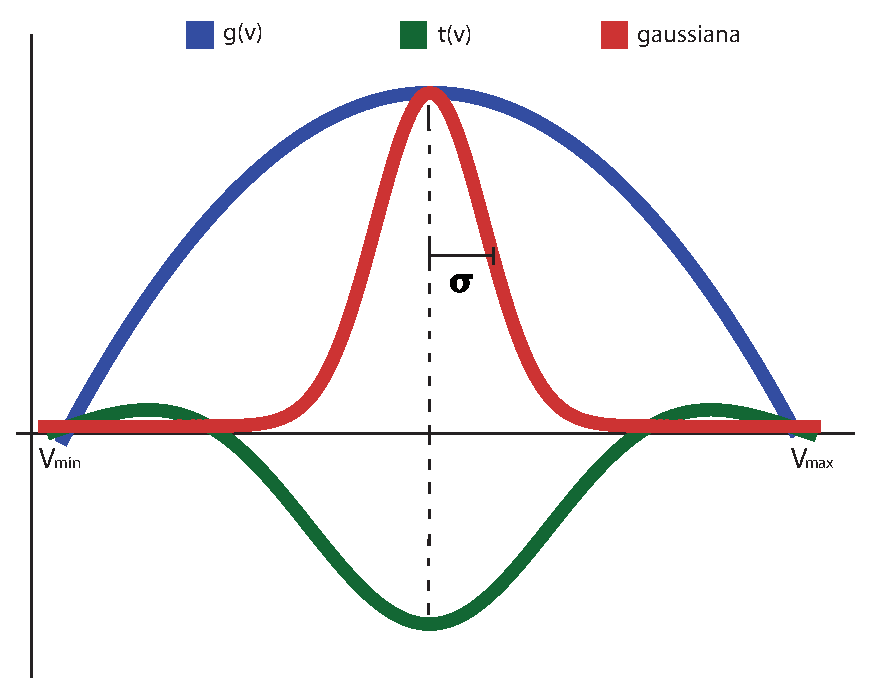
\includegraphics[width=0.7\textwidth]{images/m_gauss_ft}
		\label{fig:m_gauss_ft}
	}
	\subfigure[]
	{
		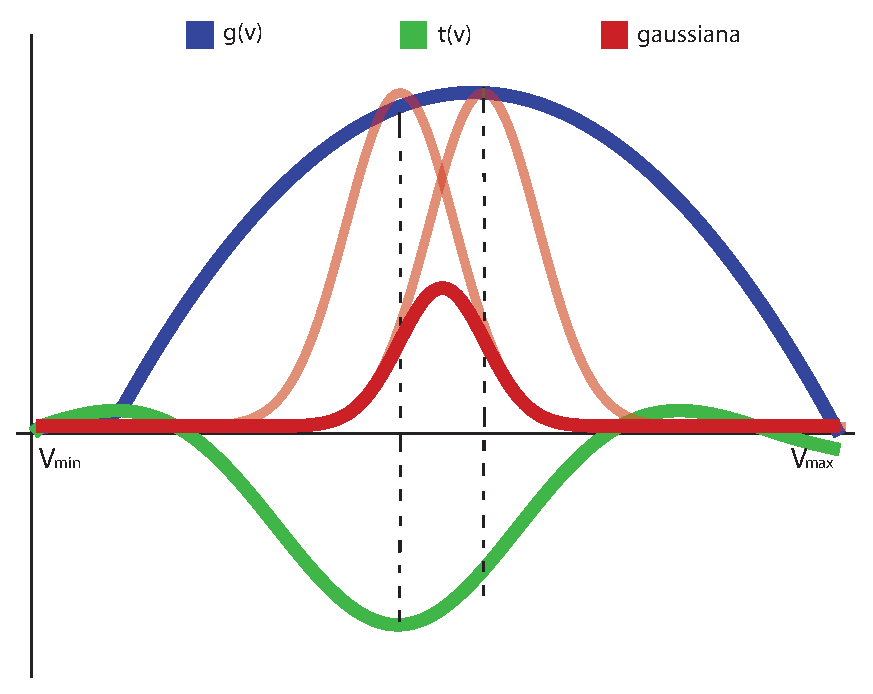
\includegraphics[width=0.7\textwidth]{images/m_gausses_ft}
		\label{fig:m_gausses_ft}
	}
	%TODO
	\label{fig:m_gauss}
	\caption{Lalala...}
\end{figure}
	
	É preciso lembrar, porém, que a expressão para a distância $ x $ ao centro da fronteira foi descartada. A posição exata de uma fronteira agora é indicada mutuamente por um máximo local em $ g(v) $ e um mínimo local em $ t(v) $. Como essas curvas são compostas de valores médios, seus extremos podem não coincidir em um mesmo $ v $. Contudo, se as fronteiras forem identificadas separadamente para cada função e suas gaussianas multiplicadas, o resultado é também uma gaussiana, que atinge seu máximo no ponto de interseção das funções que lhe deram origem. Assim é obtido um novo escalar $ v $ onde a fronteira está centrada.

	Um outro fato sobre as curvas médias é que elas raramente apresentarão o comportamento exibido nas imagens da Figura~\ref{fig:m_gauss}. Apesar de \textit{Kindlmann e Durkin}~\cite{gordon} terem demonstrado que isso é possível, o volume utilizado na demonstração possuí apenas uma fronteira e esta se comporta idealmente de acordo com o modelo proposto por eles. Nos volumes em que o intervalo de valores das fronteiras se sobrepõem, a média afeta os arcos esperados, como mostra a Figura~\ref{fig:}. Porém, as fronteiras ainda são identificadas por máximos locais em $ g(v) $ e mínimos locais em $ t(v) $. Na verdade, o formato no qual esses extremos se apresentam pode ser utilizado para inferir a \quote{força} ou importância de uma fronteira.
	
\begin{figure}[h]
	\centering
	\subfigure[]
	{
		%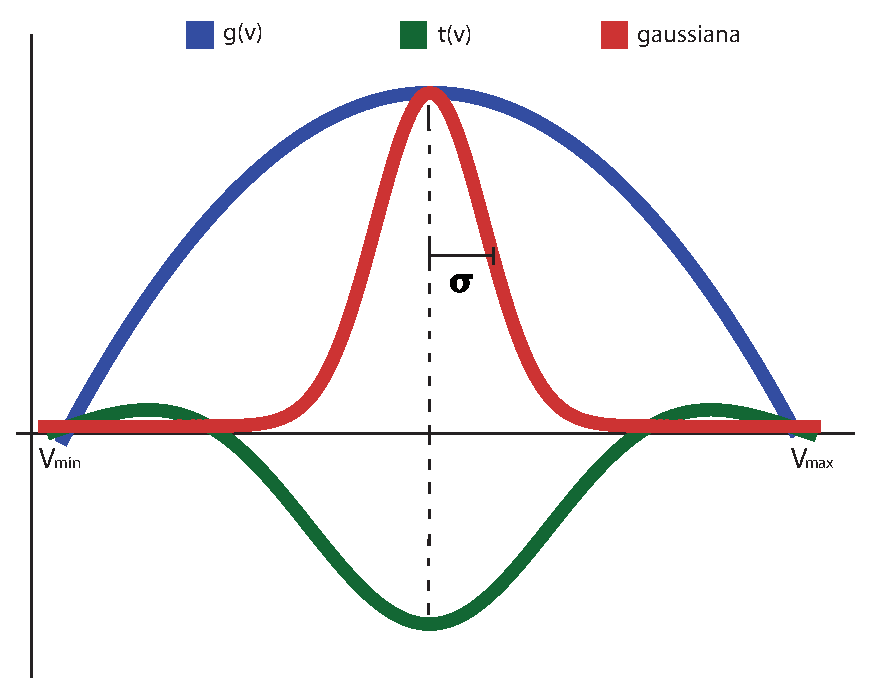
\includegraphics[width=0.7\textwidth]{images/m_gauss_ft}
		\label{fig:m_gauss_ft}
	}
	\subfigure[]
	{
		%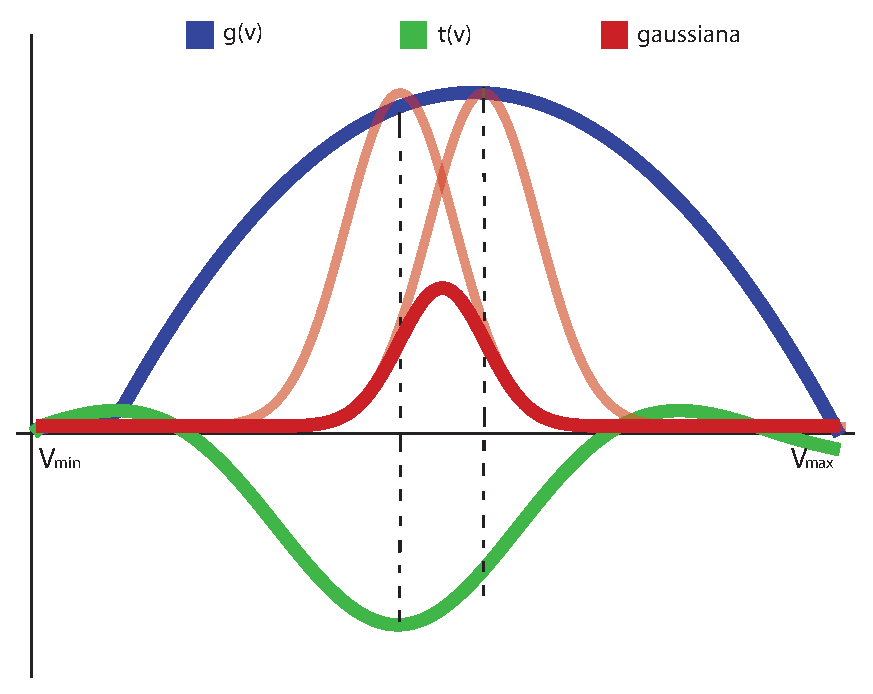
\includegraphics[width=0.7\textwidth]{images/m_gausses_ft}
		\label{fig:m_gausses_ft}
	}
	%TODO
	\label{fig:m_gauss}
	\caption{Lalala...}
\end{figure}
	
	Dois fatores indicam a \quote{força} de uma fronteira nas funções médias: a amplitude e largura do extremo local na qual ela se encontra. A amplitude claramente é um indício de \quote{força} da fronteira já que uma derivada maior implica em uma mudança de valores mais brusca. Contudo, uma variação não tão ríspida, porém longa, indica uma grande mudança de material sendo visualizado, o que justifica o uso da largura do extremo local. A largura é definida como sendo a maior distância entre o extremo local que indica o centro da fronteira e seus extremos imediatamente opostos.
	
	Então, para cada máximo local de $ g(v) $ e mínimo em $ t(v) $, a gaussiana centrada tem amplitude máxima $ A(v) $ definida pelo produto da altura com a largura desse extremo. O conjunto dessas gaussianas geradas para $ g(v) $ define a curva $ G_{g}(v) $, que é normalizada para que seu pico máximo seja sempre $ 1 $. O mesmo é feito com a função $ t(v) $, dando origem à curva $ G_{t}(v) $. A função de transferência $ FT(v) $ é dada pela multiplicação de $ G_{g}(v) $ e $ G_{t}(v) $. Por fim, a função de transferência também é normalizada e multiplicada por um fator de opacidade. Dessa forma, o usuário pode controlar a transparência da FT.
	
	Seja $ \alpha $ o fator de opacidade e $ \sigma $ a espessura da fronteira, ambos definidos pelo usuário, $ P_{g} $ o conjunto de valores escalares que apresentam máximo local em $ g(v) $ e $ P_{t} $ o conjunto de  valores escalares que apresentam mínimo local em $ t(v) $
	
\begin{equation}\label{ft}
\begin{array}{c}
	\vspace{2mm}
	G_{g}(v) = \left\lvert A(v)\right\rvert \cdot \max_{\forall p\ \in\ P_{g}}\left\{ e^{-\frac{(v-p)^{2}}{2\sigma^{2}}}\right\}
	\\
	\vspace{2mm}
	G_{t}(v) = \left\lvert A(v)\right\rvert \cdot \max_{\forall p\ \in\ P_{t}}\left\{ e^{-\frac{(v-p)^{2}}{2\sigma^{2}}}\right\}
	\\
	FT(v) = \alpha \cdot G_{g}(v) \cdot G_{g}(v)
\end{array}
\end{equation}